\documentclass[../notes.tex]{subfiles}
\graphicspath{{\subfix{../img/}}}
\begin{document}


\part{ECE352: Computer Organization}

\marginnote{Taught by Prof. Andreas Moshovos}
\section{Admin stuff}
\subsection{Lecture 1}



\begin{itemize}
	\item Lecture recordings on \href{https://tinyurl.com/2jthyk8k}{YouTube}
	\item Online notes: \href{https://www.eecg.utoronto.ca/~moshovos/ECE352-2022}{https://www.eecg.utoronto.ca/~moshovos/ECE352-2022/}
	\item Course will cover the following:
	 \begin{itemize}
	 	\item C to assembly
		\item How to build a processor that works
		\item Intro to processor optimizations
		\item Peripherals
		\item OS support (Maybe)
		\item (Maybe) Arithmetic circuits
		\item Use NIOS II and cover a little bit of RISC-V
	 \end{itemize}	
\end{itemize}



\subsubsection{Mark breakdown}

\begin{itemize}
	\item Labs 15\%
	\item project 5\%
	\item midterm  30\%
	\item Final 50\%
	\item All exams will be open notes/book/whatever except another person/service helping you.
\end{itemize}

\section{Preliminary}
\subsection{Lecture 2: Using binary quantities to represent other things}

Computers can represent information in bits; 0/1. 
Though they don't necessarily know or care what bits are, we may assign our own arbitrary meaning to them -- usually numbers with the help of positioning; the LSB represents $ 2^0 $ and so forth.

C types \marginnote{Or, just \texttt{\  ;;include <stdint.h>}...}
	\begin{itemize}
		\item int: 32b (word)
		\item char: 8b (byte)
		\item short: 16b (half word)
		\item long: 32b (word)
		\item long long: 64b
	\end{itemize}

Signed numbers may be represented in a number of ways.
\begin{itemize}
	\item Sign bit (make MSB represent positive or negative numbers and then the remaining $ n-1 $ bits represent the number. Con: hardware impl sucks because requires if/else
	\item Two's complement \sidenote{Flip bits, add one. Intuition; in 3 bit system, adding 7 to 1 would result in 8 which would get truncated to 0.}. Pro: only need to implement adders on hardware and then negative numbers will work just like any other except must be interpreted differently. Positive numbers would always start with a $ 0 $ and negatives would start with $ 1 $. So the range of possible values becomes $ -(2^{n-1}-1), +2^{n-1}-1$ 
\end{itemize}

Adding together binary numbers can also cause overflow; $ (A+B) \ge A, (A+B) \ge  B $ may not always be true.
Also, when we work with these types we always use all the bits. This has implications when working with values of different lengths.

\begin{itemize}
	\item \texttt{char b = -1}  \texttt{(1111 1111))}
	\item \texttt{short int c = -1}  \texttt{(0000 0000 0000 0001))}
	\item \texttt{a = b + c} \texttt{0000 0001 0000 0000 } 
	\item In order to deal with this we must \texttt{cast} the \texttt{char} to a \texttt{short int}. This is done via sign extension which prepends $ 0 $s or $ 1 $s \sidenote{two's complement} to the \texttt{char} so that math can be done on it.
\end{itemize}


\subsubsection{Floating Point Numbers}


Whereas fixed point numbers i.e. $ \$5.25 $ can be represented just as how an integer would be represented but with the understanding that the user would interpret it as having a decimal point somewhere that indicates the position of $ 2^0 $.
This decimal point would be the same for all numbers of that type, i.e. we could have a six bit number that has places $ 2^2 2^1 2^0 2^{-1} 2^{-2} $ 
This is common in embedded systems and how it is formatted isn't super clearly standardized.

\begin{lemma}
	Reference: \href{https://www.eecg.utoronto.ca/~moshovos/ECE352-2022/00.practice/What\%20Every\%20Computer\%20Scientist\%20Should\%20Know\%20About\%20Floating-Point\%20Arithmetic.htm}{What Every Computer Scientist Should Know About Floats}
\end{lemma}





\begin{definition}
	\textbf{IEEE 754 Floating Point}

	This is a single precision 32 bit float

	\begin{equation}
		\texttt{S  EEEEEEEE  MMMM MMMM MMMM MMMM MMMM MMM}
	\end{equation}
	

	The most significant \texttt{S} bit is the sign bit, bits 30 through 23 \texttt{E} form the exponent which is an unsigned integer, and 22 through 0 form the (\texttt{M})antissa. The number being represented can be found using the following:

	\begin{equation}
	(-1)^S \times 2 ^ {(E-127)} \times 1.\text{Mantissa}
		\label{eq:352:float32_eq}
	\end{equation}

	\begin{example}
		For example, given the following float:
		\begin{equation*}
			1\quad10000001\quad10000000000000000000000
		\end{equation*}
		
		So S = 1, E = 10000001 = 129 and Mantissa = 10000000000000000000000.
		The number is therefore

		\begin{equation}
			(-1^1) \times 2^{(129-127)} \times 1.10000000000000000000000 = -6.0
		\end{equation}
	\end{example}


	IEEE754 also defines 64 bit floating-point numbers. They behave the same except for now having an 11 bit exponent, the bias being 2047\mn{instead of 126}, and the mantissa having 52 bits\marginnote{In \texttt{c}, \texttt{float} is a 32 bit float and \texttt{double} is 64}.


	A few special cases are also available to represent other quantities

	\begin{itemize}
	\item If E=0, M non-zero, value=$(-1)^S \times 2^{-126} \times 0.M$ (denormals)
		\item If E=0, M zero and S=1, value=-0
		\item If E=0, M zero and S=0, value=0
		\item If E=1...1, M non-zero, value=NaN 'not a number`
		\item If E=1...1, M zero and S=1, value=-infinity
		\item If E=1...1, M zero and S=0, value=infinity
	\end{itemize}

	Floating-point numbers are inherently imprecise. Addition and subtract are inherently lossy; the mantissa window may not be large enough to capture the decimal points. Multiplication and division just creates a ton of numbers.
	\marginnote{There are more floating point formats introduced by nvidia and google such as a half-precision or 8-bit float designed to reduce memory use for machine learning}

	Converting real numbers to IEEE754 floats, here using 37.64 as an example, can be done as follows
	\begin{itemize}
		\item Repeatedly divide the part of the number $ >0 $ by $ 2 $ and get the remainders, i.e. 37/2 = 18, rem = 1 -> 18/2 = 0, rem = 0 -> 4/ 2 = 2, rem = 0, 2/2 = 1, rem = 0, 1/2 = 0, rem = 1. As a 2 bit number E is 100101. But we need to convert it to IEEE754 format with the exponent; E - 127 = 5, E = 132 = 1000 0100.
		\item Do the same for the part of the number past the decimal, but multiplying by two and checking if > 1: 0.64 * 2 = 1.28 -> 1, 0.28 * 2 = 0.56 -> 0, 0.56 * 2 = 1.12 -> 1 ... and so forth. At some point we will hit a cycle but we'll just take the $ N_{\text{mantissa}} $ of digits.
	\end{itemize}

	So the full number is $  0 1000 0100 0010 1101 0001 1110 1011 111 $
\end{definition}


\section{NIOS II Preliminary}


\subsection{Lecture 3: Behavioural Model of Memory}


Computers can be described as a set of units, each of which interact with each other and the outside world in a specified way.
For example, modern computers tend to have memory units, processing units, display units, and so forth.
Each unit has a set of inputs and outputs, and a set of rules that govern how the unit behaves.
This gives the manufacturer flexibility in how they want to implement a unit, as long as the unit behaves as specified.
When designing these operational units it is important to strike a balance between functionality and specificity; if the unit is too specific it will be difficult to implement, but if it is too general it will be difficult to use.

\marginnote{\textbf{Specification} is the description of what an unit should do, and \textbf{implementation} is how it actually does it. For example, an \texttt{OR} gate can be specified as a truth table and then implemented via transistors or a person in a box.}

\subsubsection{Memory}
Memory is a unit that stores information and is usually represented as a vector of elements, usually a byte (8 bites).
Each element, or memory location, contains a binary quantity and has an associated \textit{address}.
The address is a number that uniquely identifies the location of the element in the vector, and is \textbf{permanently fixed} at time of manufacture.
Most systems are byte-addressable, meaning that there is an unique address for each byte in the memory.
The collection of all addresses is called the \textbf{address space} of the memory, which is typically a power of two.
Modern systems tend to be 32 or 64 bit, meaning that the address space is $ 2^{32} $ or $ 2^{64} $ elements long.

For each memory location there there are two operations available
\begin{itemize}
	\item \textbf{Read}: Read the value stored at a given address
	\item \textbf{Write}: Write a value to a given address
\end{itemize}


Typical memory behaviour models define that the order of memory operations matters, i.e. 

\begin{enumerate}
	\item \texttt{store 0x10, 0xf0} 
	\item \texttt{store 0x20, 0xf0} 
\end{enumerate}

We would see that \texttt{0xf0} contains the value \texttt{0x20} and not \texttt{0x10} due to the sequential execution model.
Memory that adheres to the sequential model offers operations that are \textbf{atomic}; the operations are performed on its own with no interaction or overlap with anything else.



\begin{figure}[H]
	\centering
	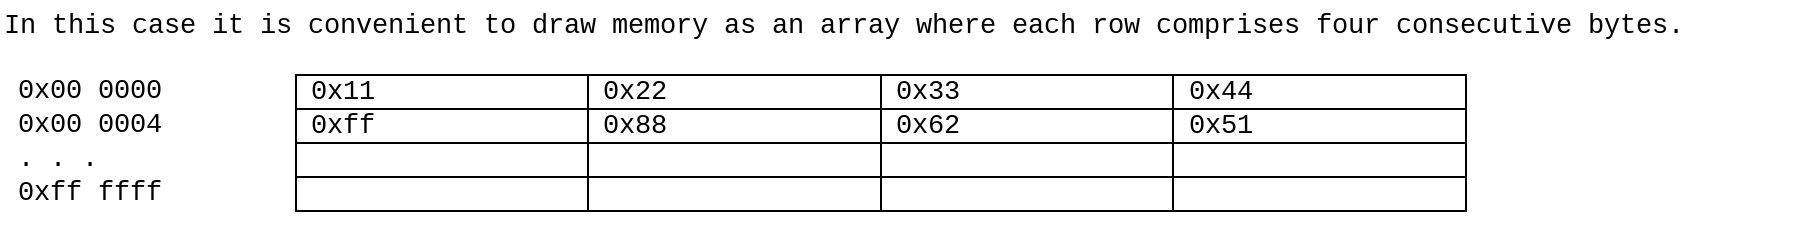
\includegraphics[width=\linewidth]{img/image_2022-09-16-02-10-27.png}
\end{figure}

Systems are generally also addressable by words, halfwords, and bytes.
Different architectures have different constraints on allowing unaligned access\sidenote{Aligned access only means to allow [only] reads or writes for a data size i.e. halfword to an address divisible by the size of said data type. For example an longword access on our development board would be at an address divisible by $ 4 $}

\textbf{Endianness} refers to the order in which bytes are stored in memory. Though some processors are big-endian, most modern processors are little-endian. The NIOS II used for this course is little-endian. 

\begin{figure}[H]
	\centering
	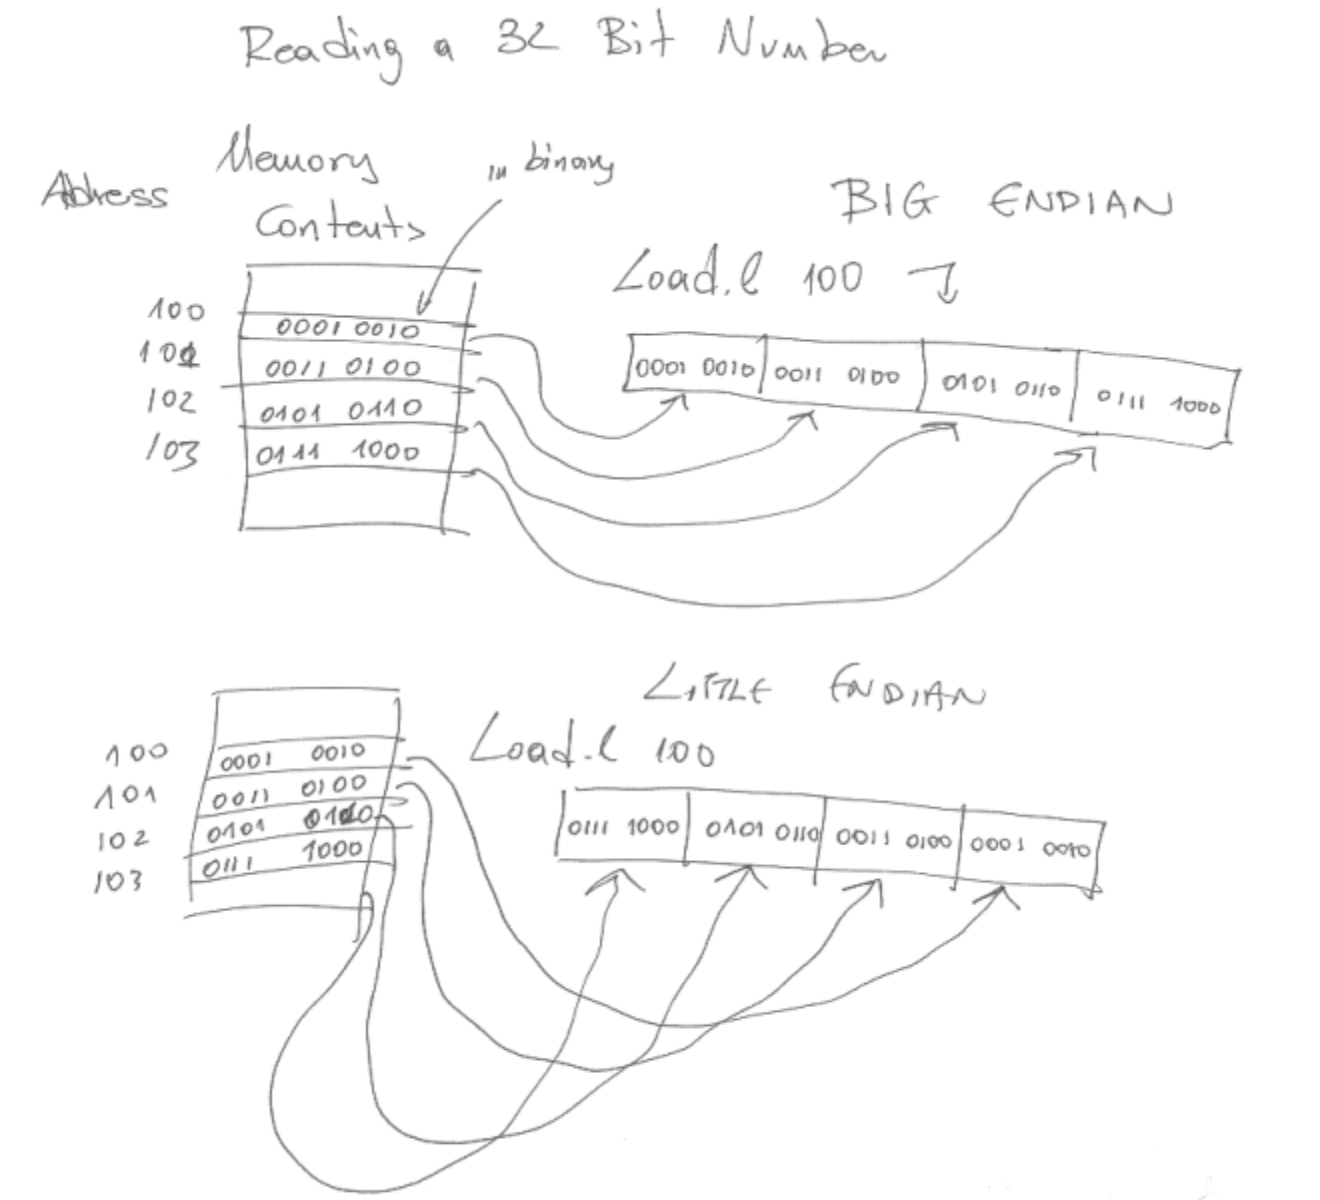
\includegraphics[width=0.8\linewidth]{img/image_2022-09-16-02-16-30.png}
\end{figure}

\subsubsection{Physical Interface}

What physical interfaces would be necessary to implement this behavioural model? 

Given a summary of requirements as follows:

\begin{enumerate}
	\item Read and write operations
	\item Addressable by byte, word, longword
	\item 24 bit address
	\item 32 bit for writing
	\item 32 bit for reading
	\item signal for do nothing
\end{enumerate}


A single bit signal can be used to indicate whether the memory is reading or writing, and a two bit signal can be used to specify if we're interested in addressing by byte, word, or longword.
The address is 24 bits, so we need 24 address lines.
As for reading/writing data, we have the option of having two 32 bit data lines, or multiplexing a single 32 bit line.
A single bit signal can be used to indicate to do nothing or not. \marginnote{The use of a single bit signal to indicate `do nothing' is necessary because a physical device won't be able to change all signals instantaneously, so we use it to tell the memory to wait until these transient effects die off}

One way of multiplexing the data lines is to use a tri-state buffer, which is a buffer that can be enabled or disabled.
When enabled, the buffer acts as a normal buffer, but when disabled, the output is disconnected from the input.
On the other hand this means that our memory chip would not support simultaneous reads or writes.




\begin{figure}[H]
	\centering
	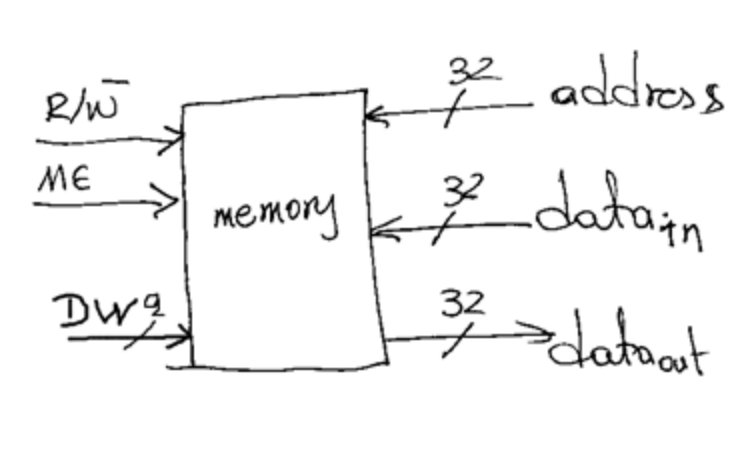
\includegraphics[width=0.8\linewidth]{img/image_2022-09-16-02-18-16.png}
\end{figure}

\subsection{Lecture 4: NIOS II Programming Model}

The NIOS II assumes a \texttt{32-bit} address space where each address holds a single byte.
Each byte is addressable, and three data types are supported. Halfword and word accesses must be aligned.

\begin{itemize}
	\item \textbf{Byte}: 8 bits
	\item \textbf{Halfword}: 16 bits
	\item \textbf{Word}: 32 bits
\end{itemize}

The NIOS II also has a set of registers

\begin{itemize}
	\item 32 general purpose 32 bit registers
		\begin{itemize}
			\item \texttt{r0} is always zero\marginnote{Many operations can be synthesized using another operation involving zero, i.e. assignment \texttt{A=B} can be implemented as \texttt{A = B + 0} }
		\end{itemize}
	\item 6 control registers, 32 bits each
	\item Program counter (PC), 32 bits
\end{itemize}

There are certain conventions for the use of registers, which are as follows:
\begin{figure}[H]
	\centering
	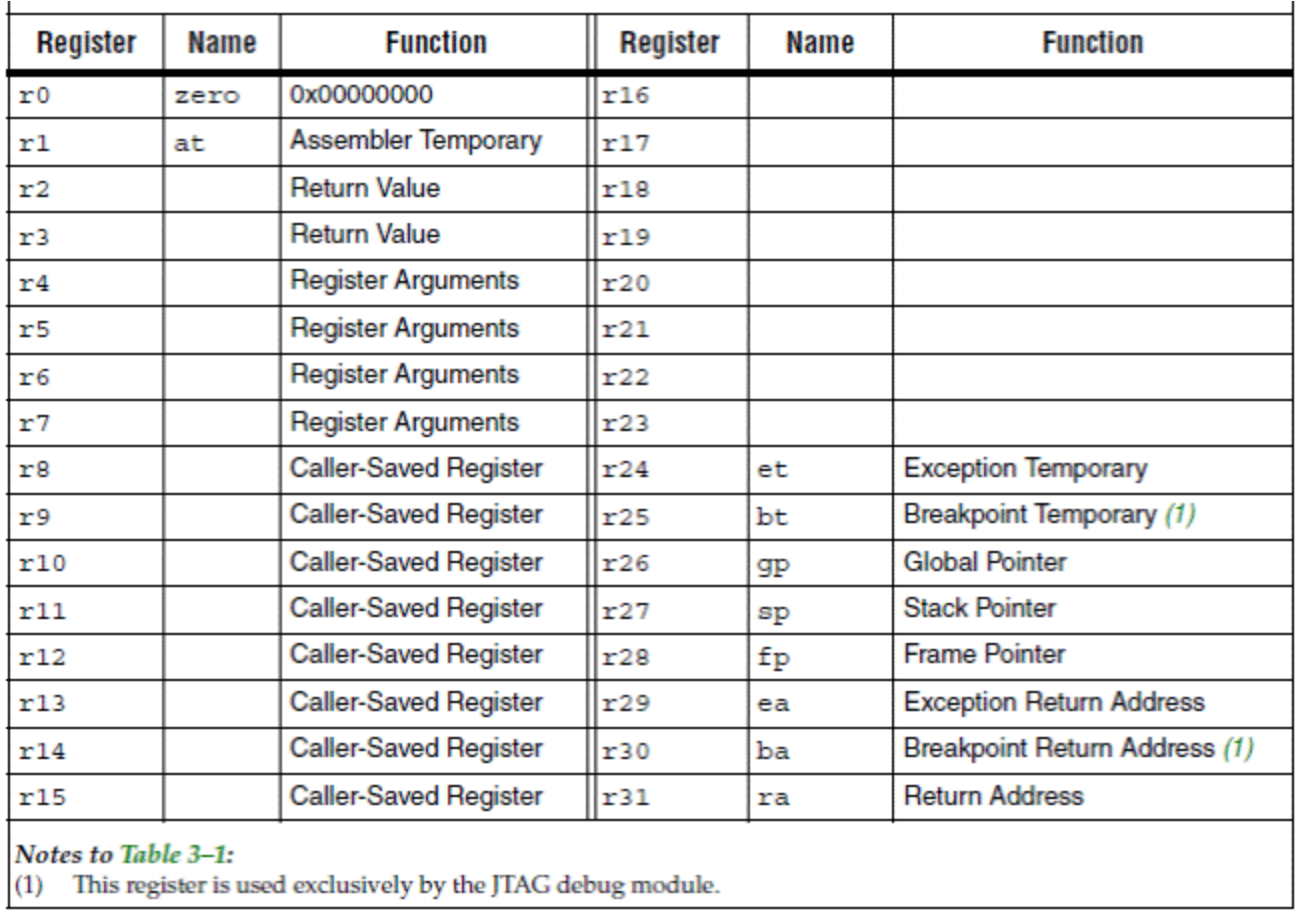
\includegraphics[width=0.8\linewidth]{img/image_2022-09-16-17-17-34.png}
\end{figure}

\subsubsection{Adding Two Numbers}
As an exercise, let's see how we can implement the following piece of code in NIOS II assembly

\begin{listing}[H]
\begin{minted}{c}
unsigned int a = 0x00000000;
unsigned int b = 0x00000001;
unsigned int c = 0x00000002;

a = b + c;
\end{minted}
\end{listing}


\textbf{Register-only version} 

\marginnote{\texttt{addi} stands for `add intermediate', the only difference being that the second operand is a number. It is used to set a constant}

\begin{listing}[H]
\begin{minted}{gas}
addi r9, r0, 0x1
addi r10, r0, 0x2
add r9, r10, r11
\end{minted}
\end{listing}

In general, most instructions take the form of \texttt{operation destination, source1, source2}.


Breaking it down even further we can see that these assembly instructions actually perform a number of steps

\begin{listing}[H]
\begin{minted}{gas}
addi r9, r0, 0x1
	; 1. read r0
	; 2. Add value read in step 1 with 0x1
	; 3. Write result of step 2 to r9
	; 4. increment PC to next instruction
addi r10, r0, 0x2
	; 1. read r0
	; 2. Add value read in step 1 with 0x2
	; 3. Write result of step 2 to r10
	; 4. increment PC to next instruction
add r9, r10, r11
	; 1. read r10
	; 2. read r11
	; 3. Add values read in steps 1 and 2
	; 4. Write result of step 3 to r8
	; 5. increment PC to next instruction
\end{minted}
\end{listing}


What about 32 bit constants? An unfortunate quirk is that \texttt{addi} only supports 16 bit constants, so we need to use \texttt{ori} to set the upper 16 bits of the register.


\begin{listing}[H]
\begin{minted}{gas}
movhi r9, 0x1122
	; Sets the upper 16 bits of r9 to 0x1122
	; and the lower 16 bits to zero
ori r9, r9, 0x3344
	; bitwise OR the value in r9 with 0x3344
	; which will set the lower 16 bits to 0x3344
\end{minted}
\end{listing}

This is a PITA so NIOS II offers a few pseudo-instructions to make this easier




\begin{listing}[H]
\begin{minted}{gas}
movi rX, Imm16
	; sets rX to the sign-extended (signed) 16 bit immediate
movui rX, Imm16
	; sets rX to a zero-extended unsigned 16 bit immediate
movia rX, Imm32
	; sets rX to a 32 bit immediate
\end{minted}
\end{listing}

{\let\thefootnote\relax\footnote{
	\begin{itemize}
		\item Footnote1: \texttt{movia} does not use the \texttt{movhi} and \texttt{ori} instructions to create a 32-bit immediate but rather a \texttt{movhi} and a \texttt{addia}.
\texttt{addi}  will sign extend it's 16-bit field so some adjustment might be needed for whatever is being passed to \texttt{movhi}.
		\item Footnote2: movhi r9, \%hi(0x11223344) is equivalent to movhi r9, 0x1122. Ori r9, \%lo(0x11223344) is equivalent to ori 9, 0x3344. That is, \%hi(Imm32) returns the upper 16-bits of Imm32 and \%lo(Imm32) the lower 16 bits.
		\item Footnote3: movhi r9, \%hiadj(0x11223344) followed by addi r1, \%lo(0x11223344) is the correct way of creating a 32-bit immediate using movhi and addi. \%hiadj(Imm32) returns the upper 16 bits of the immediate  as-is or incremented by 1 if bit 15 is 1. Think why this is necessary based on footnote 1.
		\item Footnote4: \%hi(), \%lo(), and \%hiadj() are macros supported by the assembler. They are not NIOS II instructions. They get parsed during compile time. 
	\end{itemize}
}}


\subsubsection{Adding two numbers using memory}

NIOS II is a load/store architecture which means that all data manipulation happens only in registers.


\begin{listing}[H]
\begin{minted}{gas}
; read b from memory into r9
movhi r11, 0x0020
ori   r11, r11, 0x0004
ldw   r9, 0x0(r11)

; read c from memory into r10
movhi r11, 0x0020
ori   r11, 0x0008
ldw   r10, 0x0(r11)

; add, then store into r8
add   r8, r9, r10

; store r8 into memory
movhi r11, 0x0020
ori   r11, r11, 0x0000
stw   r8, 0x0(r11)
\end{minted}
\end{listing}


The new instructions introduced here are


\begin{listing}[H]
\begin{minted}{gas}
ldw rX, Imm16(rY) ;; 'load word' from memory
;; rX, rY registers, Imm16 is a 16 bit immediate
;; TLDR; Rx = mem[rY + sign-extended(Imm16)]
; 1. read rY
; 2. sign-extend Imm16 to 32bits
; 3. adds the result of step 1 and 2
; 4. reads from memory a word (32 bit) using the result of step 3 as the address
; 5. write the result of step 4 to rX
\end{minted}
\end{listing}

\begin{listing}[H]
\begin{minted}{gas}
stw rX, Imm16(rY) ;; 'store word' to memory
;; rX, rY registers, Imm16 is a 16 bit immediate
;; TLDR; mem[rY + sign-extended(Imm16)] = rX
; 1. read rY
; 2. sign-extend Imm16 to 32bits
; 3. adds the result of step 1 and 2
; 4. write to memory rX using the result of step 3 as the address
\end{minted}
\end{listing}

This can be simplified using the \texttt{movia} macro

\begin{listing}[H]
\begin{minted}{gas}
movia r11, 0x200004
ldw   r9, 0x0(r11)
movia r11, 0x200008
ldw   r10, 0x0(r11)
add   r8, r9, r10
movia r11, 0x200000
stw   r8, 0x0(r11)
\end{minted}
\end{listing}


In this lecture so far we have seen three addressing modes

\begin{enumerate}
	\item Register addressing, i.e. \texttt{rX} 
	\item Immediate addressing, i.e. \texttt{Imm16}
	\item Register indirect addressing with displacement, i.e. \texttt{Imm16(rY)}. This is how we calculate the referenced memory address. Register indirect refers to using a register's value to refer to memory, and `displacement' refers to adding a constant prior to using the register value to access memory. Register indirect addressing is where we use a displacement of 0.
\end{enumerate}


We can exploit register indirect addressing with displacement.

\begin{listing}[H]
\begin{minted}{gas}
movhi r11, 0x0020
ori   r11, r11, 0x0004
ldw   r9, 0x0(r11)
;; can be replaced with
movhi r11, 0x0020
ldw r9, 0x4(r11)
\end{minted}
\end{listing}

Note that the value of \texttt{r11} does not change since the subsequent operations use an offset to that value.

Generally when we want to read memory from \texttt{A} we can use

\begin{listing}[H]
\begin{minted}{gas}
movhi r11, (upper 16 bits of A)
ori   r9, r11, (lower 16 bits of A)
\end{minted}
\end{listing}


Care must be taken when the 16th bit of \texttt{A}  is 1 since the addition that \texttt{ldw} performs will sign extend it to be a negative number, i.e. 

\begin{listing}[H]
	\begin{minted}{gas}
movhi r11, 0x0020
ldw r9, 0x8000(r11)
;; this is incorrect because
;; will extend to 0xFFFF8000, which would result
;; in a final address of 0x001F800
\end{minted}
\end{listing}


This is where the macros \texttt{\%hiadj(Imm32)}  and \texttt{\%lo(Imm32)} come in handy, since they will add 1 to the values if bit 15 of Imm32 is 1. 
This results in code that looks like this:


\begin{listing}[H]
	\begin{minted}{gas}
movhi r11, %hiadj(0x208000)
ldw r9, %lo(0x2080000)(r11)
;; will extend to 0xFFFF8000, which would result
;; in a final address of 0x001F800
\end{minted}
\end{listing}


\section{Assembly Basics}
\subsection{Lecture 5: Simple Control Flow}

We have prior worked with straight-line sequences.
In this lecture we will look at how to add control flow to our programs, i.e if-then-else, etc.


\marginnote{The \texttt{data} section contains stuff that you want to be initialized for you before the entry point of the program is called, e.g. global variables. This segment as a fixed size. The \texttt{text} or \texttt{code} segment contains executable instructions (typically read-only, unless the architecture allows self-modifying code) and typically resides in the lower parts of memory. \texttt{bss} contains static and global variables which are zero-initialized; usually used for uninitialized data}

A pseudo-c program will be rewritten in assembly to illustrate the concepts.

\begin{listing}[H]
\begin{minted}{c}
unsigned int a = 0x00000000;
unsigned int b = 0x11223344;
unsigned int c = 0x22334455;

if (b == 0)
then a = b + c;
else a = b – c;

\end{minted}
\end{listing}

\begin{listing}[H]
\begin{minted}{gas}
      .section .data
va:   .long 0x0
vb:   .long 0x11223344
vc:   .long 0x55667788
 

main:
      movia r11, va
      ldw   r9, 4(r11)
      beq   r9, r0, then
else:
      ldw   r10, 8(r11)
      sub   r8, r9, r10
      stw   r8, 0(r11)
      beq   r0, r0, after

then:
      ldw   r10, 8(r11)
      add   r8, r9, r10
      stwio r8, 0(r11)
after:
\end{minted}
\end{listing}
\begin{definition}

	We encounter two new instructions in this snippet.
\begin{itemize}
	\item \texttt{sub} is a subtraction instruction
	\item \texttt{beq}: a branch-if-equals instruction
\end{itemize}

The \texttt{beq} instruction takes the general form 

\texttt{beq RX, rY, label}. 

This instruction will compare the values of $ rX $ and $ rY $ and if the condition is true then the program counter will jump to the destination label. 
When the branch changes the program counter it is called a taken branch, otherwise it is non-taken. Non-taken branches fall through to the next instructions. 

\begin{blockquote}
	Note: whereas the assembly \texttt{beq} command is written as a comparison with a label to jump to, in the NIOSII instruction the destination is encoded relative to the instruction location with a 16-bit displacement constant. The displacement is therefore calculated as $ PC + 4 + \text{displacement} $, meaning that we can jump at most $ +32774, -32772 $ bytes\mn{16 bit signed constant+4, with 4-byte alignment since instructions are 4 bytes long.} from the current program counter. The compiler will complain if the branch cannot be implemented.


	Encoding is as follows: 

	\texttt{AAAAA BBBBB IIIIIIIIIIIIIIII 0x26}.

	where $ A $, $ B $ are register names (hence 5 bit), $ I $ is a 16 bit immediate value, and $ 0x26 $ is the branch type, in this case $ beq $  


	Most branches tend to be branch backwards because of loops.
\end{blockquote}


Other branch instructions include


% TODO (ihasdapie): Finish up this list & cleanup
\begin{itemize}
	\item \texttt{br}: always/unconditional branch
	\item \texttt{bne}: branch if not equal
	\item \texttt{blt}: branch if less than, w/ signed comparison
	\item \texttt{bltu}: branch if less than, w/ unsigned comparison
	\item \texttt{bgt}: branch if greater than, w/ signed comparison
	\item \texttt{bgtu}: branch if greater than, w/ unsigned comparison


\end{itemize}


\end{definition}






\begin{listing}[H]
\begin{minted}{gas}
	.data
	.align 4 ;; Align to word size addresses which are faster to access
a: .word 0
b: .word 0x11223344
c: .word 0x55667788
	.text
	movia r11, a  ;; moves the address of a into r11
	ldw r9, 4(r11) ;; loads the value at address a+4 into r9
	ldw r10, 8(r11)
	add r8, r9, r10
	stw r8, 0(r11)
\end{minted}
\end{listing}






\subsection{Lecture 6, 7: For loops and arrays}

How can we implement the following in assembly?

\begin{listing}[H]
\begin{minted}{c}
short arr[5] = { 1, 2, 3, 4, 5 }; // an array of word values (16 bit)
short n = 5;            // the number of elements in the array
short sum = 0;
 
for (i = 0; i  < n; i++)
   sum = sum + arr[i];
\end{minted}
\end{listing}


Arrays are typically implemented at the machine level as a contiguous block of memory.
\marginnote{Generally element \texttt{a[i]} is at address \texttt{\&a[0] + sizeof(TYPE) * i}    }

\begin{listing}[H]
	\begin{minted}{gas}
		.data
		.align 1
arr .hword 1,2,3,4,5
n   .hword 5
sum .hword 0
	\end{minted}
	\caption{Creating a static array in assembly}
\end{listing}

Multidimensional arrays are handled by having an array of pointers to arrays and dereferencing twice to arrive at the desired memory location.
Alternatively we can allocate a $ 1x(m \cdot  n) $ chunk of memory and then address it as $ a[i][j] = a[i \cdot n + j] $.
\marginnote{\texttt{c} and pascal and other modern programming languages store arrays in row-major order, i.e. consecutive elements in a row are place together in memory. FORTRAN uses column-major.}





As for the for loop, let's look at at what \texttt{c} does first.

\begin{listing}[H]
\begin{minted}{c}
for (init; cond; post)
	body
\end{minted}
\caption{General form of a \texttt{c} for loop}
\end{listing}


Breaking it down a little more into atomic steps


\begin{listing}[H]
\begin{minted}{c}
INIT
if (!COND), we are done
BODY
POST
GOTO line 2
\end{minted}
\caption{General form of a \texttt{c} for loop}
\end{listing}

Let's now rewrite this in assembly

\begin{listing}[H]
\begin{minted}{gas}
		.text
forloop:
	add r8, r0, r0 ;; INIT
	movia r9, n ;; set COND, i.e. the n that we compare i to. See: loop invarient :)
	ldh r9, 0(r9)
;; movhi r9, %hiadj(n)
;; ldh r9, %lo(n)(r9) ;; this code block is a shorter piece with the same effect
loop:
	bge r8, r9, endloop ;; test condition for when we are done
	;; body goes here
	;; let's use r10 to store the running sum at in the end we can load it to memory
	movia r11, arr ;; load the address of arr[0] into r11
	;; add the index to the address of arr[0]; &arr + i
	add r11, r11, r8
	;; add again; &arr + i + i = &arr + 2i
	add r11, r11, r8
	ldhio r12, 0(r11) ;; r12 = arr[i]
	add r10, r10, r12 ;; r[10] += arr[i]
	
	addi r8, r8, 1 ;; POST i.e. r8 += 1
	br loop
endloop:
	movia r11, sum
	sth r12, 0(r11) ;; write the sum to memory
\end{minted}
\end{listing}


A similar approach can be taken for while loops.


\begin{listing}[H]
\begin{minted}{gas}
.text
    
add       r8, r0, r0 ;; zero out r8
movia     r9, n ;; assumes n >= 1
ldh       r9, 0(r9) ;; loads condition
    
doloop:  
					movia r11, arr ;; grab address of arr[0]
					add  r11, r11, r8 
					add  r11, r11, r8 ;; grab addr of arr[i]
					ldh  r12, 0(r11) ;; load arr[i] into r12
					add   r10, r10, r12 ;; add arr[i] to sum
 
          addi r8, r8, 1 ;; increment i
          blt  r8, r9, doloop ;; evaluate loop condition
endloop:
          movia r11, sum
          sth  r12, 0(r11)  ;; write the sum into memory
\end{minted}
\end{listing}


\begin{blockquote}
	\texttt{gcc} is not a compiler by itself: it actually orchestrates and calls out a lot of other things

	\begin{enumerate}
	\item \texttt{cpp}: the C preprocessor, $    f.c \to  f.i $  ; dealing with \texttt{\  ;; defines}, etc. Inspect via \texttt{gcc -E} 
	\item \texttt{gcc -s f.i}: the \texttt{cc}, the c compiler $ f.i \to f.s $  : parse pure c from preprocessor and spew out assembly code
	\item \texttt{as}: the assembler, $ f.s \to f.o $:   to turn assembly to machine code, creating objects ready for linkage
	\item \texttt{ld}: the linker, $ f.o \to f $:  link together all the objects into a single executable. Looks through \texttt{LDPATH} to look for symbols to link. \mn{There is static and dynamic linking; static meaning that everything is inside. These days most are dynamically linked which can grab symbols from shared libraries (\texttt{.so}) right before/during runtime}
	\end{enumerate}
\end{blockquote}



\subsection{Lecture 8: Subroutines}

A subroutine (or how we more commonly understand them, function calls), is a way to break up a program into smaller pieces and is a core part of structured programming.

Let's look at how we can implement the following in assembly

\begin{listing}[H]
\begin{minted}{c}
int add3(int a, int b, int c){
	return a+b+c;
}
\end{minted}
\end{listing}

First, for \texttt{c}  subroutines to work as intended they must:

\begin{enumerate}
	\item Be callable from anywherei n the program
	\item Be able to pass unique parameters across different subroutine invocations
	\item Be able to return a value to the caller
	\item Must be able to change control flow such that it goes back to the point where it was called
\end{enumerate}

This leads to a number of questions:

\begin{enumerate}
	\item How does the subroutine return to the caller?
	\item how does it return a value?
	\item How do we pass arguments?
	\item What about local memory?
	\item What happens to registers when we call a subroutine?
\end{enumerate}


These issues are addressed through a set of implementation-specific (though largely universal) rules that all valid subroutines must follow. These are called \textbf{calling conventions}.



\begin{definition}
	A key concept in subroutine calling is the \textbf{stack frame}. As for how stacks work/are implemented that is a google search away.

	A stack has the following operations defined:

		\begin{enumerate}
			\item push: put a value on the top of the stack
			\item pop: remove the top value from the stack
			\item peek (distance): look at the value at a certain distance from the top of the stack
		\end{enumerate}

\end{definition}


	The NIOS II stores it's stack pointer, or the address to the top of the stack, in \texttt{r27}, i.e. the stack pointer \texttt{sp}.
	The \texttt{sp}  starts at the top of the stack (highest address value) and then the stack grows downwards to lower addresses.\sn{Conversely the heap (commonly used for dynamic memory allocation) grows upwards towards higher addresses. The stack and heap are commonly implemented such that they grow towards each other}
	There is no way to represent an empty stack in NIOS II; \texttt{r27} will always contain a valid pointer address.
	\sidenote{An element is in the stack if it's address is greater than \texttt{sp} }


\begin{definition}
	\textbf{push}  
	\begin{listing}[H]
	\begin{minted}{gas}
	;; push r9 -> stack
	subi sp, sp, 4 ;; grow stack by a long word
	;; (recall: grow downwards)
	stw r9, 0(sp) ;; save value of r9 to sp
	\end{minted}
	\end{listing}


	\textbf{pop}  
	\begin{listing}[H]
	\begin{minted}{gas}
	;; pop top of stack and return to r9
	ldw r9, 0(sp) ;; read top value
	addi sp, sp, 4 ;; increment sp; remove top elem
	\end{minted}
	\end{listing}

	\textbf{top}  
	\begin{listing}[H]
	\begin{minted}{gas}
	// access ith elem, assuming index in r9
	add r9, r9, r9 ;; assume r9 contains nedex
	add r9, r9, r9 // r9 = 4 * i
	add r9, sp, r9 ;; sp + 4*i
	ldw r9, 0(r9) // return value of ith element into r9
	\end{minted}
	\end{listing}
\end{definition}


\textbf{Calling a subroutine and having it return to the caller}  


\marginnote{\texttt{r31} is commonly used as the return address pointer and is aliased as \texttt{ra} }
The stack is used to implement this behaviour.
If a function will be calling another it has to save the \texttt{ra}  value on the stack in the beginning and restore it from the stack prior to returning.

Consider the following pseudo \texttt{c} code

\begin{listing}[H]
\begin{minted}{c}
boo_calls(){
	coo();
	doo();
	return;
}

coo(){
	doo();
	return;
}
doo(){
	return;
}
\end{minted}
\end{listing}

The NIOS II code would be as follows

\marginnote{Note that \texttt{ret} transfers execution to the address in \texttt{ra}  }
\begin{listing}[H]
\begin{minted}{gas}

	.text
boo:  ;; boo will be making calls, so it first pushes the ra value on the stack   
	subi sp, sp, 4  
	stw ra,0(sp)  ;; push the return address onto the stack


	call coo  ;; resume execution at coo, ra = PC + 4 = boo_ret1
boo_ret1:
	call doo  ;; continue execution at doo, ra = PC + 4 = boo_ret2

boo_ret2:                                        
	ldw  ra, 0(sp)  ;; pop return address from the stack
	addi sp, sp, 4
	ret  ;; resume execution at ra, which would be the return address from the 
	;; stack we just popped
coo:
	subi  sp, sp, 4 
	stw   ra,0(sp)  ;; push the return address onto the stack
	call  doo  ;; resume execution at coo, ra = PC + 4 = coo_ret

coo_ret:
	ldw  ra, 0(sp)  ;; pop return address of boo from the stack
	addi sp, sp, 4
	ret  ;; resume execution there

doo:  ;; doo will not be making any calls, no need to save ra on the stack
	ret  ;; just return to whoever called 
\end{minted}
\end{listing}





\begin{figure}[H]
	\centering
	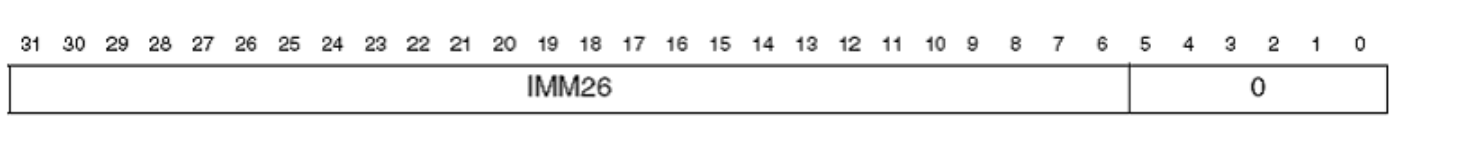
\includegraphics[width=0.8\linewidth]{img/image_2022-09-26-14-48-27.png}
	\caption{The call instruction accepts a label as the 2nd argument which is encoded as a 26 bit immediate. This limits the called function to be within 256 MB of the caller; the actual target is the immediate multiplied by 4 and then concatenating with the program counter, i.e. $ PC_{31\ldots28} = IMM26 * 4 $ }
\end{figure}

Note: we can look at executables with \texttt{objdump -d}. 

Example:


\begin{listing}[H]
\begin{minted}{c}

#include <stdio.h>
int main () {
	printf("hello world");
}

\end{minted}
\end{listing}

\begin{listing}[H]
\begin{minted}{gas}

hello_world:     file format elf64-x86-64


Disassembly of section .init:

0000000000001000 <_init>:
    1000:	f3 0f 1e fa          	endbr64
    1004:	48 83 ec 08          	sub    $0x8,%rsp
    1008:	48 8b 05 c1 2f 00 00 	mov    0x2fc1(%rip),%rax        # 3fd0 <__gmon_start__@Base>
    100f:	48 85 c0             	test   %rax,%rax
    1012:	74 02                	je     1016 <_init+0x16>
    1014:	ff d0                	call   *%rax
    1016:	48 83 c4 08          	add    $0x8,%rsp
    101a:	c3                   	ret

Disassembly of section .plt:

0000000000001020 <printf@plt-0x10>:
    1020:	ff 35 ca 2f 00 00    	push   0x2fca(%rip)        # 3ff0 <_GLOBAL_OFFSET_TABLE_+0x8>
    1026:	ff 25 cc 2f 00 00    	jmp    *0x2fcc(%rip)        # 3ff8 <_GLOBAL_OFFSET_TABLE_+0x10>
    102c:	0f 1f 40 00          	nopl   0x0(%rax)

0000000000001030 <printf@plt>:
    1030:	ff 25 ca 2f 00 00    	jmp    *0x2fca(%rip)        # 4000 <printf@GLIBC_2.2.5>
    1036:	68 00 00 00 00       	push   $0x0
    103b:	e9 e0 ff ff ff       	jmp    1020 <_init+0x20>

Disassembly of section .text:

0000000000001040 <_start>:
    1040:	f3 0f 1e fa          	endbr64
    1044:	31 ed                	xor    %ebp,%ebp
    1046:	49 89 d1             	mov    %rdx,%r9
    1049:	5e                   	pop    %rsi
    104a:	48 89 e2             	mov    %rsp,%rdx
    104d:	48 83 e4 f0          	and    $0xfffffffffffffff0,%rsp
    1051:	50                   	push   %rax
    1052:	54                   	push   %rsp
    1053:	45 31 c0             	xor    %r8d,%r8d
    1056:	31 c9                	xor    %ecx,%ecx
    1058:	48 8d 3d da 00 00 00 	lea    0xda(%rip),%rdi        # 1139 <main>
    105f:	ff 15 5b 2f 00 00    	call   *0x2f5b(%rip)        # 3fc0 <__libc_start_main@GLIBC_2.34>
    1065:	f4                   	hlt
    1066:	66 2e 0f 1f 84 00 00 	cs nopw 0x0(%rax,%rax,1)
    106d:	00 00 00 

		;; and this goes on for a while loading in the .so & printf
\end{minted}
\end{listing}


And more assembly later ... 



\begin{listing}[H]
\begin{minted}{gas}

0000000000001139 <main>:
    1139:	55                   	push   %rbp
    113a:	48 89 e5             	mov    %rsp,%rbp
    113d:	48 8d 05 c0 0e 00 00 	lea    0xec0(%rip),%rax        # 2004 <_IO_stdin_used+0x4>
    1144:	48 89 c7             	mov    %rax,%rdi
    1147:	b8 00 00 00 00       	mov    $0x0,%eax
    114c:	e8 df fe ff ff       	call   1030 <printf@plt>
    1151:	b8 00 00 00 00       	mov    $0x0,%eax
    1156:	5d                   	pop    %rbp
    1157:	c3                   	ret

Disassembly of section .fini:

0000000000001158 <_fini>:
    1158:	f3 0f 1e fa          	endbr64
    115c:	48 83 ec 08          	sub    $0x8,%rsp
    1160:	48 83 c4 08          	add    $0x8,%rsp
    1164:	c3                   	ret


\end{minted}
\end{listing}

























\subsection{Lecture 9}

We've seen how to call and return from subroutines -- but what about passing arguments and returning values?
\marginnote{The following calling convention is the one used by gcc for the NIOS II family}
For this lecture we'll assume that only words are returned from and passed to subroutines, but other data types and structs can be used as well.


\begin{itemize}
	\item Return value is passed in \texttt{r2}\mn{only one return value can be given; multiple can be encoded via structures or ptrs etc}
	\item First four parameters are passed in \texttt{r4, r5, r6, r7} 
	\item Additional parameters are pushed onto the stack \textit{in order} 
		\begin{itemize}
			\item We push the last argument to the stack first and so forth such that the first non-register argument (the 5th one) is the first to be popped off once we enter the function.
		\end{itemize}
\end{itemize}

Consider a function which takes seven integers and adds them together.

\begin{listing}[H]
\begin{minted}{gas}
	.data
sum: .word 0
	.text
main:

addi sp, sp, -4
stw ra, 0(sp);
;; return address ptr (ra) is pushed onto the stack

;; fill first 4 args
movi r4, 1
movi r5, 2
movi r6, 3
movi r7, 4

;; allocated for arguments 5-7
addi sp, sp, -12 ;; 3 words * 4 byte


;; push arguments 5-7 onto the stack
;; note order; <top> 5, 6, 7
movi r2, 7
stw r2, 8(sp)

movi r2, 6
stw r2, 4(sp)

movi r3, 5
stw r2, 0(sp)

call add7

add7:
	add r2, r4, r5    # add the first two arguments and place the sum into r2
	add r2, r2, r6    # add the third argument to r2
	add r2, r2, r7    # add the fourth argument to r2
	ldw r7, 0(sp)     # read the fifth argument from the stack
	add r2, r2, r7    # add to r2
	ldw r7, 4(sp)     # read the sixth argument from the stack
	add r2, r2, r7    # add to r2
	ldw r7, 8(sp)     # read the seventh argument from the stack
	add r2, r2, r7    # add to r2 (return value in r2 by convention)
	 ret
;; and then do the cleanup etc
\end{minted}
\end{listing}

Note that in reality \texttt{gcc}   will actually preallocate all the memory needed by the function before the function is called. So instead of allocating 12 bytes (3x 1 word arguments) as it does on line 17, it will actually allocate 16 bytes because we need to store the return address.

The allocated stack frame for the function will be the largest of any function being called from it.

For example,

\begin{listing}[H]
\begin{minted}{c}
int main(){
	foo(1,2,3);
	boo(1,2,3,4,5,6,7,8);
}
\end{minted}
\end{listing}

Boo has the maximum number of arguments, so we'll need to allocate $ 8-4=4 $ words on the stack for the arguments and the return address -- $5*4=20$ bytes. This results in

\begin{listing}[H]
\begin{minted}{gas}
;; prologue
addi sp, sp, -20
stw, ra, 16(s0)  ;; note little-endian and remaining 16 bytes for 4 argument words

;; epilogue
ldw ra, 16(sp) // pop return addr from stack
addi sp, sp, 20;
\end{minted}
\end{listing}












\subsection{Lecture 10: Recursive Subroutines}

Consider this code block that computes the Ackerman function


\begin{listing}[H]
\begin{minted}{c}
int Ackerman(unsigned int x, unsigned int y)
{
	if (x==0) return y+1;
	if (y==0) return Ackerman(x-1, 1);
	return Ackerman(x-1, Ackerman(x, y-1));
}
\end{minted}
\end{listing}

This function is interesting to implement because of it's recursive nature.


Breaking it down a little more,
\begin{listing}[H]
\begin{minted}{c}
int Ackerman(unsigned int x, unsigned int y)
{
	if (x==0) return y+1;
	if (y==0) return Ackerman(x-1, 1);
	int tmp = Ackerman(x, y-1)
	return Ackerman(x-1, tmp);
}
\end{minted}
\end{listing}


The return address and the value of \texttt{x} must be stored on the stack, so we will need space for 2 words.


\begin{listing}[H]
\begin{minted}{gas}
	.text
Ackerman:
	addi sp, sp, -8
	stw ra, 4(sp)

	bne r4, r0, Xnot0;
Xis0:
	addi r2, r5, 1
	br epilogue
Xnot0:
	bne r5, r0, Ynot0
Yis0:
	;; pass arguments
	addi r4, r4, -1 ;;First one is x-1, i.e. r4-1
	addi r5, r0, 1 ;; second is 1
	call Ackerman
	br epilogue
Ynot0:
	stw r4, 0(sp) ;; perserve value of x on the stack
	;; x is already at the right place for fn call
	addi r5, r5, -1 ;; decrement y
	add r5, r5, 0
	call Ackerman
epilogue:
	ldw ra, 4(s0)
	addi sp, sp, 8
	ret
\end{minted}
\end{listing}









\subsection{Lecture 11: Structs and recursive structures}
Consider a binary tree with a left and right child and a value. We can represent this as a struct in C.


\begin{listing}[H]
\begin{minted}{c}
struct node{
	int value;
	struct node *left;
	struct node *right;
};
\end{minted}
\end{listing}

The memory layout of the struct is word-aligned and \textit{exactly} like that of the struct definition. In this case value lives as addr+0, left at addr+4, and right at addr+8. 



\marginnote{When this gets compiled note that in memory the struct will be word-aligned, i.e. on a 4-byte word machine the beginning of the struct will be at an address which is a multiple of the word size}

Now, consider the following recursive function to perform binary search on a BST

\begin{listing}[H]
\begin{minted}{c}
int findv(int d, struct node) {
	struct node * m;
	m = root;
	if (root == NULL) {
		return 0;
	}
	if (root->val == d) {
		return 1;
	}
	if (d <= root->v) {
		return findv(d, root->left);
	}
	else {
		return findv(d, root->right);
	}
	// Note that this is a tail-recursive function, i.e. 
	// nothing is done after the recursive call
	// some compilers may unfurl this into a loop
}
\end{minted}
\end{listing}

How can we represent this in assembly?


\begin{listing}[H]
\begin{minted}{gas}
// int d is in r4, root is in r5 (by convention)
	.text

findv:
	addi sp, sp, -4
	stw R4, 0(sp);
isrootnull:
	bne r5, r0, isdv
rootisnull:
	movi r2, 0
	br epilogue
isdv:
	ldw r2, 0(r5) ;; r2 <- root->val
	bne r2, r4, tryagain
found:
	mov r2, 1
	br epilogue
tryagain:
	ble r4, r2, goleft
goleft:
	ldw r5, 4(r5) ;; offset struct addr pointer to right member
	call findv
	br end 
goright:
	ldw r5, 8(r5) ;; offset struct addr pointer to right member
	call findv
	br end
notfound:
	add r2, r0, r0
epilogue:
	ldw ra, 0(sp)
	addi sp, sp, +4
	ret
\end{minted}
\end{listing}

\subsection{Lecture 12: Devices}


A computer is great and all, but for it to be useful it must communicate with the outside world via devices. A simple device interface is the Parallel Port Interface, a common implementation of which is the GPIO (General Purpose Input/Output) interface\sn{Of which the NIOS II board has two}

There are two registers used to communicate with the NIOSII GPIO interface which live in memory;

\begin{itemize}
	\item \texttt{dr}  (data register) at \texttt{0xFF200060} 
	\item \texttt{dir}  (data register) at \texttt{0xFF200064} 
\end{itemize}

\texttt{dr} is the data word to communicate in and out of the GPIO interface, and \texttt{dir} denotes if the signal is an input or an output. Note that the \texttt{stwio} and \texttt{ldwio} variants of the \texttt{stw} and \texttt{ldw} instructions must be when interfacing with IO devices



\begin{figure}[H]
	\centering
	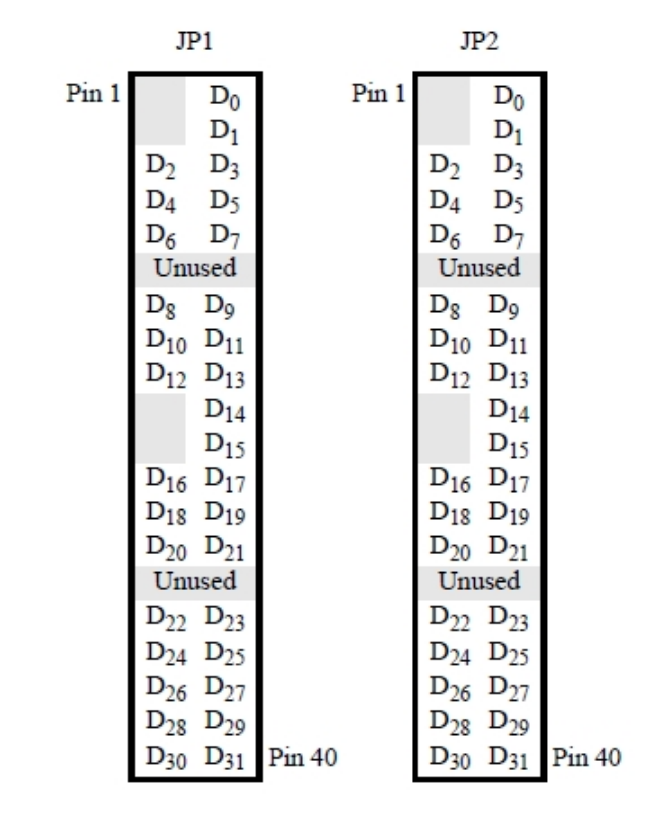
\includegraphics[width=0.8\linewidth]{img/image_2022-10-06-13-47-12.png}
	\caption{GPIO pinout}
\end{figure}


Two exercises we will cover include building a thermostat with the GPIO pins and building a keyboard. 









\subsection{Lecture 12}


\end{document}

% 352 END
